\section{编译器与系统优化}
\label{sec:system_optimization}

在模型压缩与算法优化之后，下一步是将 LLM 编译并部署到硬件设备上。
为了实现高效推理，可采用多类编译器优化。
同时，随着模型规模增大，部署常需多设备协同，形成复杂推理基础设施，系统级优化因此成为热点。
本节讨论常见编译/系统优化技术，包括算子融合、内存管理、负载卸载与并行服务。

\subsection{算子融合}

\begin{figure}[t]
    \centering
    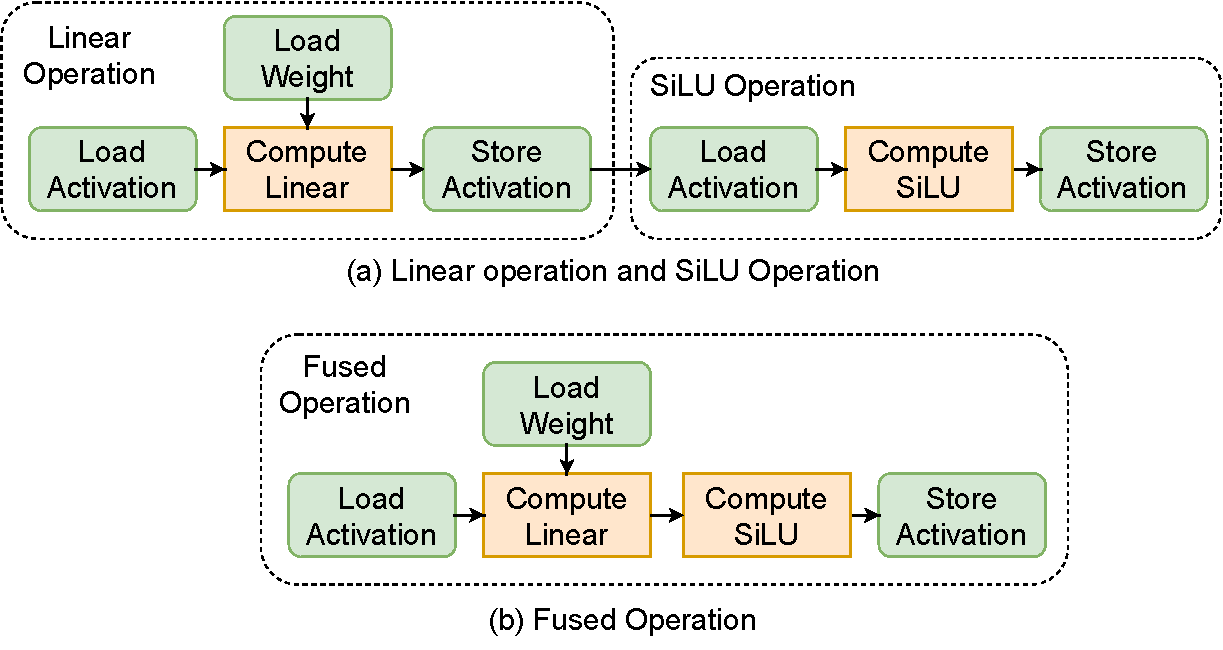
\includegraphics[width=0.95\linewidth]{ims/operator_fusion.pdf}
    \caption{线性算子与 SiLU 融合示意。}
    \label{fig:operator_fusion}
\end{figure}

\begin{figure}[t]
    \centering
    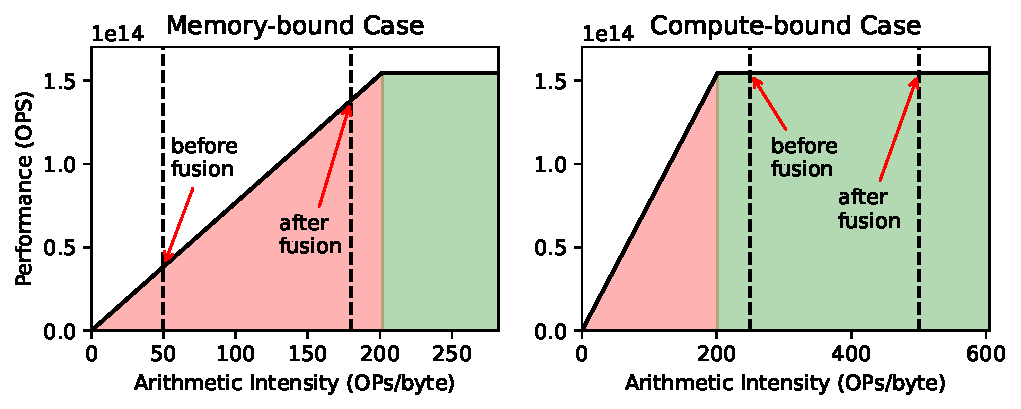
\includegraphics[width=0.95\linewidth]{ims/roofline_operator_fusion.pdf}
    \caption{算子融合在 memory-bound 与 compute-bound 场景下的差异。}
    \label{fig:roofline_operator_fusion}
\end{figure}

\begin{figure}[t]
    \centering
    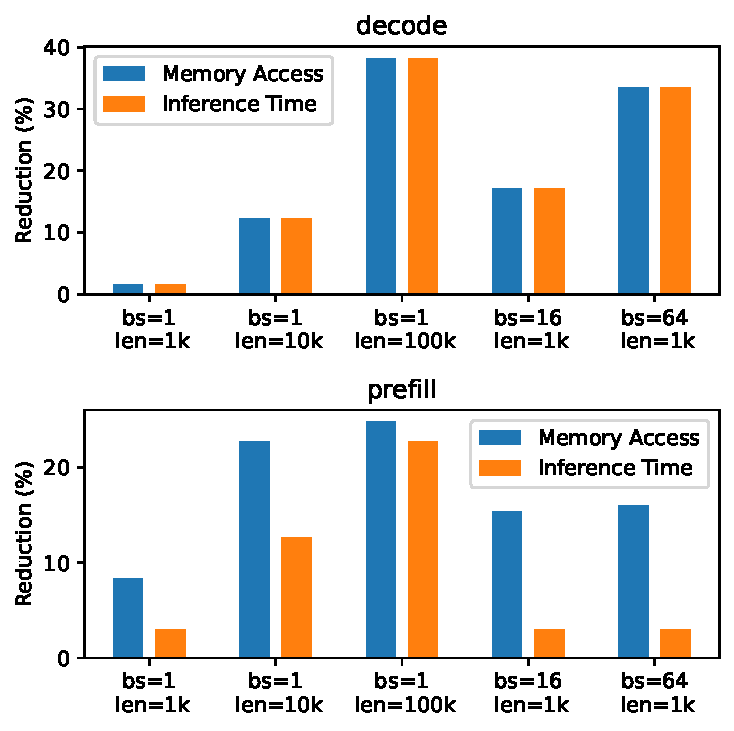
\includegraphics[width=0.95\linewidth]{ims/flashattention_reduction.pdf}
    \caption{FlashAttention 在 Nvidia A6000 上的访存与时延下降效果。}
    \label{fig:flashattention_reduction}
\end{figure}

算子融合是深度学习编译阶段的重要优化手段。
它将计算图中直接相连的多个算子合并执行，从而减少中间结果写回与重复读写。
例如“Linear + SiLU”可融合为单核执行（图~\ref{fig:operator_fusion}）。
这种方式可降低内存占用与访存开销。

Roofline 视角下（图~\ref{fig:roofline_operator_fusion}），融合通常提升算术强度，对 memory-bound 区域收益明显；
若算子已处于 compute-bound 区域，融合收益会较小。

但融合并非总可行：
(1) 若中间结果还被其它分支使用，直接融合会引入额外复杂度；
(2) 融合后片上缓冲需求可能变大，受限于硬件 on-chip buffer 容量；
(3) 框架与硬件实现本身可能对可融合模式有限制。

TVM~\citep{chen2018tvm} 等编译器可自动识别并执行融合。
对 LLM 而言，由于网络结构固定，常更适合采用手工设计的融合模式。
典型例子是注意力融合：
FlashAttention~\citep{dao2022flashattention,dao2023flashattention2} 与 Flash-Decoding~\citep{dao2023flashdecoding} 将注意力中的 MatMul 与 softmax 融合，避免显式存取庞大注意力矩阵。
图~\ref{fig:flashattention_reduction} 显示其可显著减少访存与时延。
值得注意的是 decode 阶段“访存下降约等于时延下降”，而 prefill 阶段时延收益略小于访存收益，原因是 prefill 存在部分 compute-bound 算子。

其它代表性系统包括：
DeepSpeed-Inference 的 Deep-Fusion~\citep{aminabadi2022deepspeedinference}、
xFormers~\citep{xFormers2022} 的融合 softmax/linear/layer norm/SwiGLU、
TensorRT-LLM~\citep{vaidya2023tensorrt_llm} 的模式匹配融合。

除了融合，算子内核本身也可进一步优化。
例如 FlashDecoding++~\citep{hong2023flashdecoding++} 通过异步 softmax、flat GEMM 与双缓冲进一步提升效率。

\subsection{内存管理与负载卸载}

LLM 推理中输入与输出 token 长度常动态变化：
prefill 的序列长度随用户 prompt 变化，decode 随生成逐步增长。
这使激活张量形状不同于静态网络，内存管理复杂度上升。

PagedAttention~\citep{kwon2023efficient} 将 KV cache 分块管理：
每条序列的 KV 由多个固定 token 数块组成，并通过映射表把逻辑块映射到 GPU 物理块，机制类似 CPU 虚拟内存。

\begin{figure}[t]
    \centering
    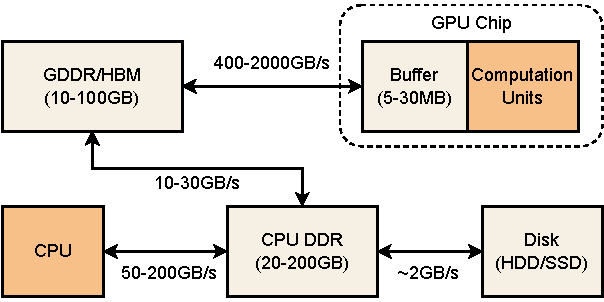
\includegraphics[width=0.9\linewidth]{ims/computer_arch.pdf}
    \caption{典型计算机体系中的分层内存空间。}
    \label{fig:computer_arch}
\end{figure}
\begin{figure}[t]
    \centering
    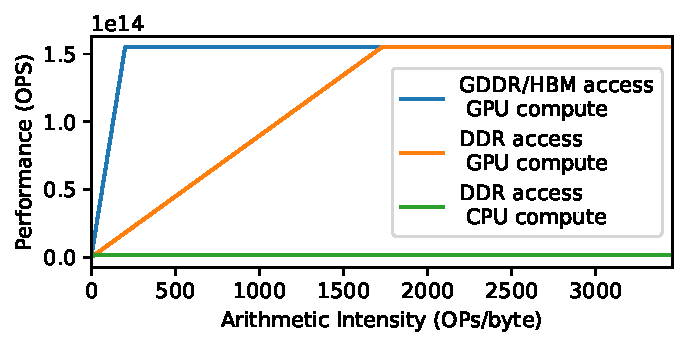
\includegraphics[width=0.9\linewidth]{ims/offloading_roofline.pdf}
    \caption{不同卸载设置下的 Roofline 模型。}
    \label{fig:offloading_roofline}
\end{figure}

当 GPU 显存不足以容纳模型时，可采用 workload offloading。
如图~\ref{fig:computer_arch}，系统通常含 CPU DDR、GPU GDDR/HBM、磁盘等不同内存层级，带宽差异显著。
图~\ref{fig:offloading_roofline} 表明：把数据存于 CPU 内存并按需传输到 GPU 计算，通常优于直接在 CPU 上计算。
当 batch 足够大时，算术强度提升，GPU 更易发挥算力。

DeepSpeed-Inference~\citep{aminabadi2022deepspeedinference} 的 ZeRO-Inference 将大模型权重卸载到 CPU，并在大 batch 下通过计算与取数重叠提升效率。
HuggingFace Accelerate~\citep{huggingface2022-accelerate} 支持将部分模块迁移到 CPU/磁盘。
FlexGen~\citep{sheng2023flexgen} 在 GPU/CPU/磁盘约束下用线性规划搜索最优吞吐策略。
\citet{alizadeh2023llminflash} 则利用闪存大容量特性，将参数驻留闪存并按需搬运到 DRAM。

\subsection{并行服务（Parallel Serving）}

并行服务面向“同时处理多用户请求”。
目标一是低延迟（单请求响应快），目标二是高吞吐（单位时间处理更多请求）。
系统需在吞吐与延迟之间做平衡。

Batching 是提升吞吐的基础手段。
图~\ref{fig:parallel_serving} 显示 decode 阶段增大 batch 可显著提升吞吐，但也会增大响应延迟与内存开销。

\begin{figure}[t]
    \centering
    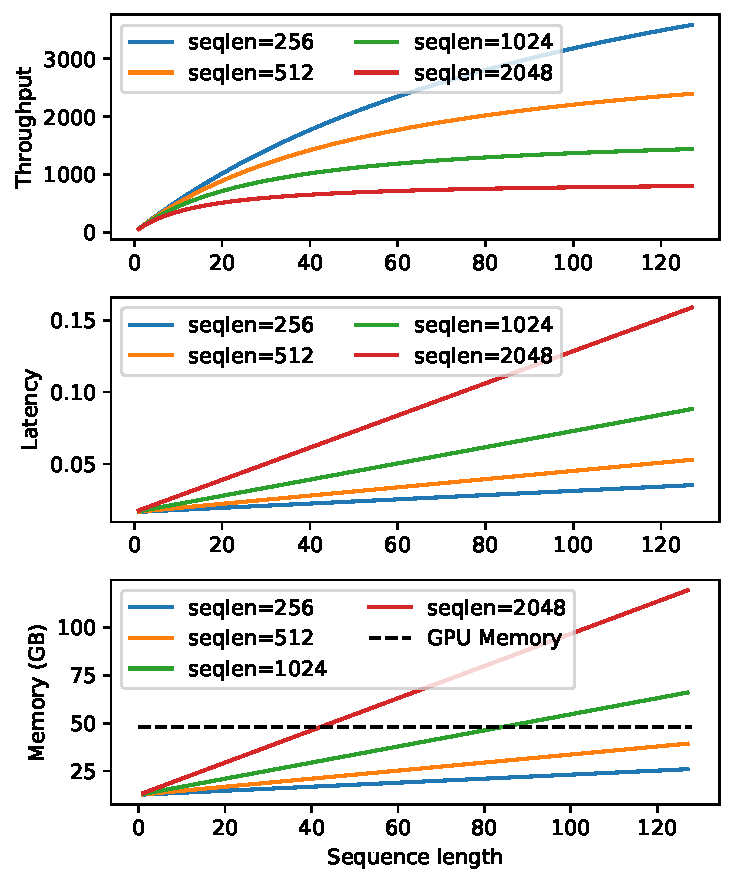
\includegraphics[width=0.9\linewidth]{ims/parallel_serving.pdf}
    \caption{并行服务策略对 Nvidia A6000（Llama-2-13b）的吞吐、时延和内存影响。}
    \label{fig:parallel_serving}
\end{figure}

为优化 batching，已有多项改进：
ORCA~\citep{yu2022orca} 提出 continuous/rolling batching；
SARATHI~\citep{agrawal2023sarathi} 提出 chunked-prefill 与 decode-maximal batching；
DeepSpeed-FastGen~\citep{holmes2024deepspeedfastgen} 与 LightLLM~\citep{modeltc2024lightllm} 也采用 split-and-fuse 思路提升稳定性与吞吐。
